\documentclass[border=1cm]{standalone}

\usepackage{tikz}
\usetikzlibrary{shapes.geometric, shapes.misc}
\usetikzlibrary{cd, fit, calc}
\usetikzlibrary{positioning}
\usetikzlibrary{decorations.markings}
\usepackage{medl_colors}
\usepackage{graphicx} %package to manage images
\graphicspath{ {./images/} } 

\usepackage{arrayjob}

\begin{document}
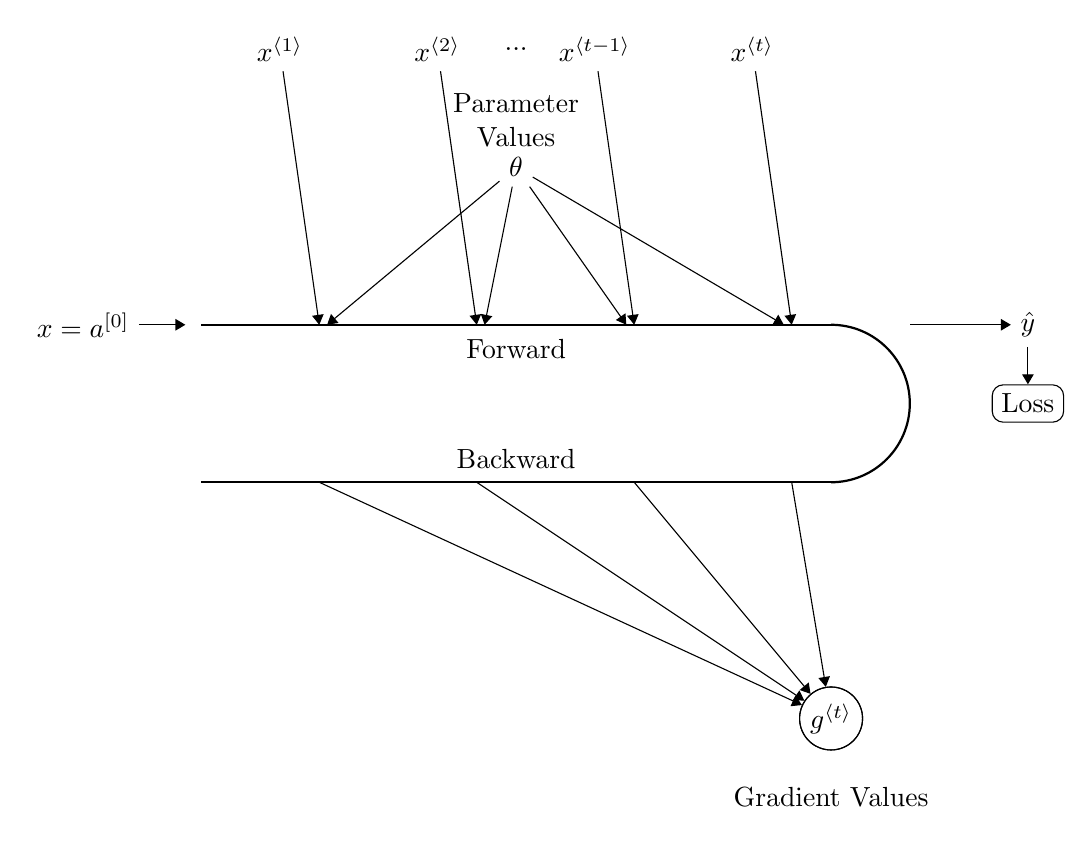
\begin{tikzpicture}

\draw[thick] (-4,0) -- (4, 0);
\draw[thick] (-4,2) -- (4, 2);
\draw[thick] (4,0) arc[start angle=-90, end angle=90, radius=1cm];

\node[] at (-3, 5.5) (t1) {$x^{\langle 1 \rangle}$};
\node[] at (-1, 5.5) (t2) {$x^{\langle 2 \rangle}$};
\node[] at (0, 5.5) (t21) {$...$};
\node[] at (1, 5.5) (t3) {$x^{\langle t-1 \rangle}$};
\node[] at (3, 5.5) (t4) {$x^{\langle t \rangle}$};
\node[] at (0, 4) (t5) {$\theta$};
% \draw[thick] (-4, 3.8) -- (4, 3.8);

\draw[-Triangle] (t1) -- (-2.5, 2);
\draw[-Triangle] (t2) -- (-.5, 2);
\draw[-Triangle] (t3) -- (1.5, 2);
\draw[-Triangle] (t4) -- (3.5, 2);

\draw[-Triangle] (t5) -- (-2.4, 2);
\draw[-Triangle] (t5) -- (-.4, 2);
\draw[-Triangle] (t5) -- (1.4, 2);
\draw[-Triangle] (t5) -- (3.4, 2);

% \node[] at (-2, -3) (b1) {$g^{\langle 1\rangle}$};
% \node[] at (0, -3) (b2) {$g^{\langle 2\rangle}$};
% \node[] at (1, -3) (b21) {$...$};
% \node[] at (2, -3) (b3) {$g^{\langle t-1\rangle}$};
\node[] at (4, -3) (b4) {$g^{\langle t\rangle}$};

\node [draw, circle, minimum size=.8cm] at (4, -3) (circle1) {};

% \draw[Triangle-] (b1) -- (-2.5, 0);
% \draw[Triangle-] (b2) -- (-.5, 0);
% \draw[Triangle-] (b3) -- (1.5, 0);
\draw[Triangle-] (circle1) -- (3.5, 0);
\draw[Triangle-] (circle1) -- (-2.5, 0);
\draw[Triangle-] (circle1) -- (-.5, 0);
\draw[Triangle-] (circle1) -- (1.5, 0);


\node[] at (-5.5, 2) (t1) {$x = a^{[0]}$};
\node[] at (6.5, 2) (t2) {$\hat{y}$};
\node[below of=t2, node distance=1cm, draw, rounded corners] (t3) {Loss};
\node [draw, circle, minimum size=.8cm] at (4, -3) {};

\draw[-Triangle] (t1) -- ++(1.3, 0);
\draw[Triangle-] (t2) -- ++(-1.5, 0);
\draw[-Triangle] (t2) -- (t3);

\node[align=center] at (0, 4.6) (tt1) {Parameter\\Values};
\node[] at (0, 1.7) (tt1) {Forward};
\node[] at (0, .3) (tt1) {Backward};
\node[] at (4, -4) (tt1) {Gradient Values};



\end{tikzpicture}
\end{document}
